\chapter{Các Kết Quả Thí Nghiệm}
\ifpdf
    \graphicspath{{Chapter4/Chapter4Figs/PNG/}{Chapter4/Chapter4Figs/PDF/}{Chapter4/Chapter4Figs/}}
\else
    \graphicspath{{Chapter4/Chapter4Figs/EPS/}{Chapter4/Chapter4Figs/}}
\fi
\label{chap_4}
\begin{quote}
\textit{Trong chương này, chúng tôi trình bày các kết quả thí nghiệm để đánh giá các đề xuất đã được nói ở chương trước. Bộ dữ liệu được dùng để tiến hành các thí nghiệm là bộ MNIST (bộ ảnh chữ số viết tay gồm các chữ số từ 0 đến 9). Các kết quả thí nghiệm cho thấy khi huấn luyện ``Sparse Rectified Auto-Encoders'' (SRAEs) với chuẩn L1 sẽ gặp phải vấn đề nơ-ron ``ngủ'', và chiến lược ``ngủ - đánh thức'' trong thuật toán ``Sleep-Wake Stochastic Gradient Descent'' (SW-SGD) của chúng tôi có thể giúp khắc phục vấn đề này. Các kết quả thí nghiệm cũng cho thấy cách ràng buộc trọng số đề xuất của chúng tôi cho kết quả tốt nhất trong số các cách ràng buộc trọng số có thể áp dụng cho SRAEs. Cuối cùng, thí nghiệm cũng cho thấy SRAEs với hai đề xuất trên của chúng tôi (SW-SGD và cách ràng buộc trọng số) có thể học được những đặc trưng cho kết quả phân lớp tốt khi so sánh với các loại ``Auto-Encoders'' khác.}
\end{quote}
\section{Các thiết lập thí nghiệm}
Chúng tôi tiến hành các thí nghiệm trên bộ dữ liệu MNIST \cite{MNIST}; bộ dữ liệu này gồm các ảnh xám (có kích thước $28 \times 28$) của mười chữ số viết tay từ 0 đến 9. Ở hình \ref{fig_MNIST} là một số ảnh mẫu của bộ dữ liệu này. Dữ liệu được tiến hành tiền xử lý bằng cách lấy mỗi giá trị điểm ảnh chia cho $255$ để đưa về đoạn $[0, 1]$. Chúng tôi sử dụng cách phân chia thường được sử dụng cho bộ dữ liệu này: $50000$ ảnh dùng để huấn luyện, $10000$ ảnh dùng để chọn các siêu tham số (validation), và $10000$ ảnh dùng để kiểm tra (test).

\begin{figure}
	\centering
	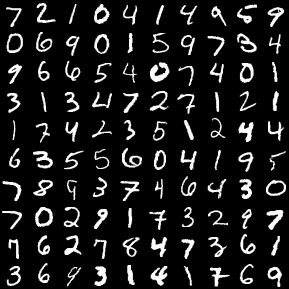
\includegraphics{MNIST}
	\caption{Một số ảnh mẫu của bộ dữ liệu MNIST}
	\label{fig_MNIST}
\end{figure}

Chúng tôi sử dụng ngôn ngữ lập trình Theano \cite{bergstra+al:2010-scipy} bởi vì ngôn ngữ này cho phép dễ dàng cài đặt các thuật toán và dễ dàng sử dụng GPU (Graphical Processing Units) để tính toán song song. Loại GPU mà chúng tôi sử dụng là NVIDIA GTX 560.

Sau khi tiến hành xong bước học đặc trưng không giám sát, chúng tôi đánh giá các đặc trưng học được bằng cách sử dụng chúng để huấn luyện mô hình phân lớp ``Softmax Regression'' và đo độ lỗi phân lớp. Một cách cụ thể, cho tập huấn luyện $\{(x^{(1)}, y^{(1)}), \ldots, (x^{(N)}, y^{(N)})\}$ với $x^{(i)} \in \mathbb{R}^{D_x}$ là véc-tơ điểm ảnh và $y^{(i)} \in \{0, \ldots, 9\}$ là nhãn lớp. Sau khi ``Auto-Encoder'' đã được huấn luyện trên tập không có nhãn $\{x^{(1)}, \ldots, x^{(N)}\}$, ta lần lượt đưa từng véc-tơ $x^{(i)}$ vào ``Auto-Encoder'' và thu được ở tầng ẩn véc-tơ đặc trưng tương ứng $h^{(i)}$; bằng cách này, ta có được tập huấn luyện mới $\{(h^{(1)}, y^{(1)}), \ldots, (h^{(N)}, y^{(N)})\}$. Kế đến, tập huấn luyện mới này được sử dụng để huấn luyện ``Softmax Regression''. Để dự đoán nhãn lớp cho một véc-tơ đầu vào mới $x_{test}$, đầu tiên ta sử dụng ``Auto-Encoder'' đã được huấn luyện để tính véc-tơ đặc trưng tương ứng $h_{test}$; sau đó đưa $h_{test}$ này vào ``Softmax Regression'' đã được huấn luyện để tính giá trị nhãn lớp dự đoán.

Trong cả hai giai đoạn học không giám sát và có giám sát, chúng tôi sử dụng thuật toán để để cực tiểu hóa hàm chi phí là Stochastic Gradient Descent (SGD) với kích thước của ``mini-batch'' là $100$ mẫu huấn luyện. Chiến lược ``dừng sớm'' (early stopping) được sử dụng để quyết định số vòng lặp (epoch) của SGD cũng như là để chống vấn đề quá khớp (trong giai đoạn học không giám sát, chúng tôi dừng quá trình tối ưu hóa dựa vào giá trị của hàm chi phí trên tập ``validation''; còn trong giai đoạn học có giám sát, chúng tôi dựa vào độ lỗi phân lớp trên tập ``validation''). Trong tất cả các thí nghiệm dưới đây, chúng tôi dùng SRAEs với $1000$ nơ-ron ẩn, tham số ``thỏa hiệp'' giữa độ lỗi tái tạo và độ thưa $\lambda$ bằng $0.25$, hệ số học khi học không giám sát bằng $0.05$, và hệ số học khi học có giám sát bằng $1$ (số lượng nơ-ron ẩn được chọn theo \cite{rifai2011HCAEs}, các siêu tham số còn lại được chọn dựa vào thực nghiệm).
\section{SGD và SW-SGD}
Để thấy được vấn đề gặp phải khi huấn luyện SRAEs với ràng buộc thưa bằng chuẩn L1 cũng như là tác dụng của chiến lược ``ngủ - đánh thức'' của chúng tôi, trong phần này chúng tôi so sánh việc huấn luyện SRAEs bằng thuật toán ``Stochastic Gradient Descent'' (SGD) và phiên bản điều chỉnh của chúng tôi, ``Sleep-Wake Stochastic Gradient Descent'' (SW-SGD). Trong thí nghiệm này, cách ràng buộc trọng số đề xuất của chúng tôi được sử dụng ($W^{(d)} = (W^{(e)})^T$, và các dòng của $W^{(e)}$ và các cột của $W^{(d)}$ được chuẩn hóa).

Hình \ref{fig_SGDvsSWSGD} thể hiện số lượng nơ-ron ``ngủ'' của SRAEs trong khi thực hiện quá trình tối ưu hóa hàm chi phí với SGD và SW-SGD. Vấn đề gặp phải khi huấn luyện SRAEs với chuẩn L1 là trong quá trình tối ưu hóa, chuẩn L1 có thể đẩy các véc-tơ trọng số đi vào các nơ-ron ẩn vào trạng thái ``ngủ'' (nghĩa là, nơ-ron ẩn tương ứng luôn cho giá trị đầu ra bằng 0 với tất cả các mẫu huấn luyện) và sau đó, chúng sẽ không bao giờ còn được cập nhật nữa. Như có thể thấy từ hình \ref{fig_SGDvsSWSGD}, khi sử dụng SGD, số lượng nơ-ron ``ngủ'' tăng dần trong quá trình tối ưu hóa, đặc biệt là trong những vòng lặp đầu tiên, khi mà quá trình tối ưu hóa vẫn còn chưa ổn định. Vấn đề nơ-ron ``ngủ'' này của chuẩn L1 có thể được khắc phục một cách đơn giản bằng chiến lược ``ngủ - đánh thức'' của chúng tôi; quá trình tối ưu hóa của SW-SGD kết thúc mà không có nơ-ron ``ngủ'' nào cả.
\begin{figure}
	\centering
	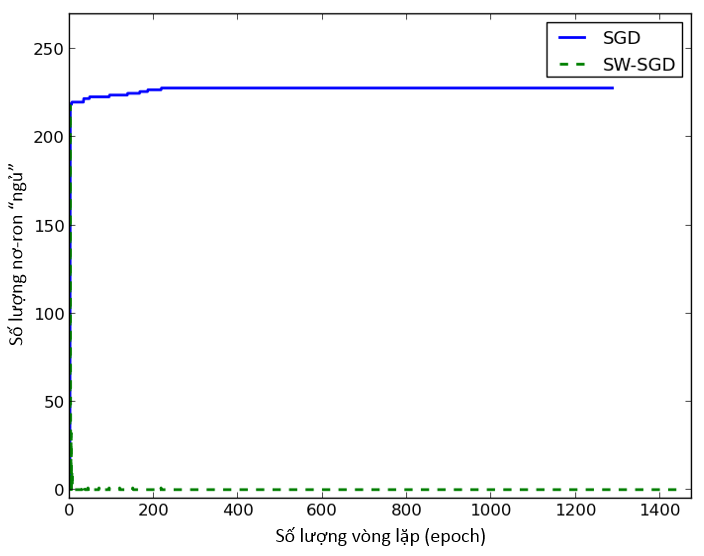
\includegraphics[width=0.8\textwidth]{SGD_vs_SW-SGD}
	\caption[So sánh giữa SGD với SW-SGD]{Số lượng nơ-ron ``ngủ'' của SRAEs trong khi thực hiện quá trình tối ưu hóa với SGD và với SW-SGD. Quá trình tối ưu hóa của SGD kết thúc với 228 nơ-ron ``ngủ'' trong tổng số 1000 nơ-ron; trong khi đó, SW-SGD kết thúc mà không có nơ-ron nào ``ngủ''. (Hai quá trình tối ưu hóa của SGD và SW-SGD kết thúc sau các số lượng vòng lặp khác nhau là do chiến lược ``dừng sớm''.)}
	\label{fig_SGDvsSWSGD}
\end{figure}

Ở hình \ref{fig_filters} là một số bộ lọc (một bộ lọc tương ứng với véc-tơ trọng số đi vào một nơ-ron ẩn) học được bởi SGD và SW-SGD. Như ta có thể thấy, với SGD, có 5 nơ-ron ``ngủ''; các bộ lọc của chúng nhìn vô nghĩa. Với SW-SGD, không có nơ-ron nào ``ngủ''; tất cả các bộ lọc đều nhìn có nghĩa, mỗi bộ lọc dò tìm một đường nét nào đó của chữ số.
\begin{figure}
	\centering
	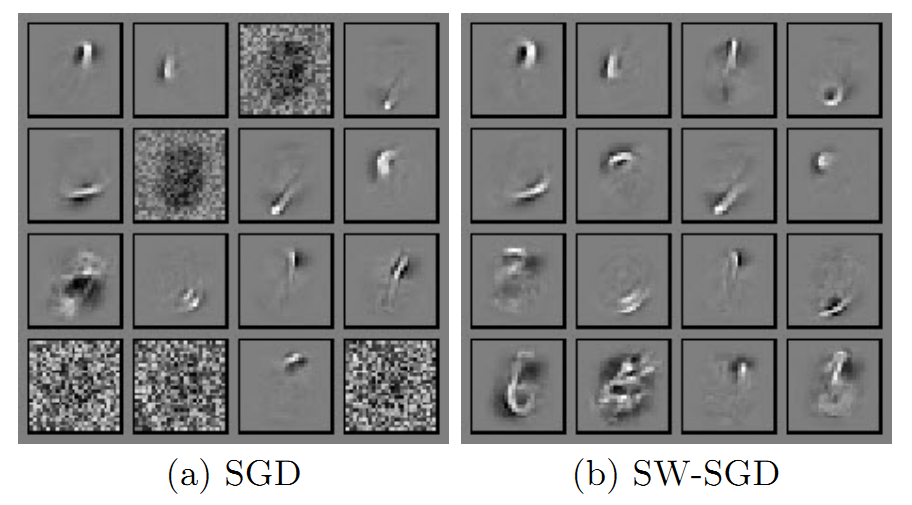
\includegraphics[width=\textwidth]{some_filters}
	\caption[So sánh giữa các bộ lọc học được bởi SGD với SW-SGD]{Ở hình (a) là một số bộ lọc (một bộ lọc tương ứng với véc-tơ trọng số đi vào một nơ-ron ẩn) học được bởi SGD; ta có thể thấy có 5 bộ lọc nhìn vô nghĩa tương ứng với 5 nơ-ron ``ngủ''. Còn ở hình (b) là các bộ lọc học được bởi SW-SGD; tất cả các bộ lọc đều nhìn có nghĩa, mỗi bộ lọc dò tìm một đường nét nào đó của chữ số.}
	\label{fig_filters}
\end{figure}

Nhờ sử dụng hết tất cả các nơ-ron ẩn, SW-SGD tìm được giá trị cực tiểu của hàm chi phí của SRAEs trên tập huấn luyện tốt hơn so với SGD; và các đặc trưng học được của SW-SGD cũng cho kết quả phân lớp (với ``Softmax Regression'') trên tập kiểm tra tốt hơn so với SGD (bảng \ref{table_SGDvsSW-SGD}).

\begin{table}
	\centering
	\caption[So sánh giữa SGD với SW-SGD]{Giá trị hàm chi phí của SRAEs trên tập huấn luyện và độ lỗi phân lớp (với ``Softmax Regression'') trên tập kiểm tra khi huấn luyện SRAEs với SGD và với SW-SGD.}
	\label{table_SGDvsSW-SGD}
	\begin{tabular}{|c|c|c|} \hline
	 & SGD & SW-SGD\\ \hline
	Giá trị hàm chi phí của SRAEs trên tập huấn luyện & 9.84 & \textbf{9.48}\\ \hline 
	Độ lỗi phân lớp trên tập kiểm tra (\%) & 1.70 & \textbf{1.62}\\ \hline
	\end{tabular}
\end{table}

\section{Cách ràng buộc trọng số đề xuất của chúng tôi và các cách ràng buộc trọng số khác}
Trong thí nghiệm thứ hai này, cách ràng buộc trọng số đề xuất cho SRAEs của chúng tôi được so sánh với các cách ràng buộc trọng số khác mà có thể áp dụng cho SRAEs. Cụ thể ở đây, chúng tôi so sánh với các cách ràng buộc trọng số sau:
\begin{itemize}
	\item \textbf{$W^{(d)}$ được chuẩn hóa:} các véc-tơ cột của $W^{(d)}$ được ràng buộc là chuẩn hóa (có độ dài bằng 1); mỗi véc-tơ cột của $W^{(d)}$ tương ứng với véc-tơ trọng số đi ra ở mỗi nơ-ron ẩn.
	\item \textbf{$W^{(e)}$ và $W^{(d)}$ được chuẩn hóa:} các véc-tơ dòng của $W^{(e)}$ và các véc-tơ cột của $W^{(d)}$ được ràng buộc là chuẩn hóa (có độ dài bằng 1); mỗi véc-tơ dòng của $W^{(e)}$ và mỗi véc-tơ cột của $W^{(d)}$ lần lượt tương ứng với véc-tơ trọng số đi vào và véc-tơ trọng số đi ra ở mỗi nơ-ron ẩn.
	\item \textbf{$W^{(d)} = (W^{(e)})^T$:} $W^{(e)}$ và $W^{(d)}$ được ràng buộc là chuyển vị của nhau.
\end{itemize}
Cách ràng buộc trọng số của chúng tôi là kết hợp của hai ràng buộc: $W^{(e)}$ và $W^{(d)}$ được chuẩn hóa, và $W^{(d)} = (W^{(e)})^T$. Trong thí nghiệm này, chúng tôi dùng SW-SGD để huấn luyện SRAEs.

Như có thể thấy ở bảng \ref{table_OurWConstraintVSOtherWConstraints}, trong số các cách ràng buộc trọng số, cách ràng buộc của chúng tôi giúp SRAEs học được những đặc trưng cho kết quả phân lớp (với ``Softmax Regression'') tốt nhất trên tập kiểm tra. Ngoài ra, bảng \ref{table_OurWConstraintVSOtherWConstraints} cũng so sánh thời gian huấn luyện SRAEs trên một vòng lặp (ứng với một lần duyệt qua toàn bộ các mẫu huấn luyện) với các cách ràng buộc trọng số khác nhau này (do chiến lược ``dừng sớm'', quá trình huấn luyện SRAEs với các cách ràng buộc khác nhau có thể kết thúc sau các số lượng vòng lặp khác nhau; do đó, để chính xác, ta nên so sánh theo thời gian huấn luyện xét trên một vòng lặp hơn là tổng thời gian huấn luyện). Các cách ràng buộc trọng số được sắp xếp theo thứ tự thời gian huấn luyện (trên một vòng lặp) tăng dần là: $W^{(d)} = (W^{(e)})^T$ (2 giây), $W^{(d)}$ được chuẩn hóa (3 giây), cách ràng buộc trọng số của chúng tôi (4 giây), $W^{(e)}$ và $W^{(d)}$ được chuẩn hóa (5 giây). Thứ tự này là hợp lý:
\begin{itemize}
	\item Ràng buộc $W^{(d)} = (W^{(e)})^T$ có thời gian huấn luyện nhanh nhất vì SRAEs không phải thực hiện bước chuẩn hóa.
	\item Ràng buộc $W^{(d)}$ được chuẩn hóa có thời gian huấn luyện lâu hơn vì bộ giải mã của SRAEs phải thực hiện bước chuẩn hóa khi lan truyền tiến; và do đó, khi lan truyền ngược, việc tính toán các đạo hàm riêng theo các tham số của bộ giải mã cũng sẽ tốn thời gian hơn bình thường.
	\item Ở cách ràng buộc trọng số của chúng tôi, khi lan truyền tiến, mặc dù cần phải thực hiện bước chuẩn hóa ở cả bộ mã hóa và bộ giải mã, nhưng nhờ vào ràng buộc $W^{(d)} = (W^{(e)})^T$, ta chỉ cần phải thực hiện bước chuẩn hóa cho bộ trọng số của bộ mã hóa, rồi sau đó dùng lại bộ trọng số đã được chuẩn hóa này cho bộ giải mã. Thời gian huấn luyện của cách ràng buộc này lâu hơn cách ràng buộc $W^{(d)}$ được chuẩn hóa ở trên vì khi lan truyền ngược, ngoài việc tính toán các đạo hàm riêng theo các tham số của bộ giải mã đã được chuẩn hóa, ta cũng cần phải tính toán các đạo hàm riêng theo các tham số của bộ mã hóa đã được chuẩn hóa (khi bộ mã hóa hay bộ giải mã phải thực hiện bước chuẩn hóa khi lan truyền tiến thì việc tính toán các đạo hàm riêng theo các tham số của chúng khi lan truyền ngược sẽ lâu hơn so với khi không thực hiện bước chuẩn hóa).
	\item Ràng buộc $W^{(e)}$ và $W^{(d)}$ được chuẩn hóa có thời gian huấn luyện lâu nhất vì khi lan truyền tiến, ta phải thực hiện bước chuẩn hóa riêng cho bộ mã hóa và bộ giải mã; và khi lan truyền ngược, ta phải tính toán các đạo hàm riêng theo các tham số của bộ giải mã và bộ mã hóa đã được chuẩn hóa.
\end{itemize}
Mặc dù thời gian huấn luyện (trên một vòng lặp) của cách ràng buộc trọng số của chúng tôi là khá cao khi so sánh với cách ràng buộc trọng số khác, nhưng nhìn chung nó vẫn nhanh (nhờ vào việc sử dụng GPU để tính toán song song). Tổng thời gian huấn luyện là khoảng 2.5 giờ.
\begin{table}
	\centering
	\caption[So sánh giữa cách ràng buộc trọng số của chúng tôi với các cách ràng buộc trọng số khác]{So sánh giữa cách ràng buộc trọng số cho SRAEs của chúng tôi với các cách ràng buộc trọng số khác mà có thể áp dụng cho SRAEs. Cách ràng buộc trọng số của chúng tôi giúp SRAEs học được những đặc trưng mà cho kết quả phân lớp (với ``Softmax Regression'') tốt nhất trên tập kiểm tra. Ngoài ra, thời gian huấn luyện trên một vòng lặp của SRAEs với các cách ràng buộc trọng số khác nhau cũng được trình bày ở cột cuối cùng của bảng.}
	\label{table_OurWConstraintVSOtherWConstraints}
	\begin{tabular}{|c|c|c|} \hline
	\textbf{Cách ràng buộc trọng số} & \textbf{\pbox{20cm}{Độ lỗi phân lớp \\trên tập kiểm tra (\%)}} & \textbf{\pbox{20cm}{Thời gian huấn luyện \\của một vòng lặp (giây)}}\\ \hline\hline
	$W^{(d)}$ được chuẩn hóa & 3.28 & 3\\ \hline
	$W^{(e)}$ \& $W^{(d)}$ được chuẩn hóa & 2.51 & 5\\ \hline
	$W^{(d)} = (W^{(e)})^T$ & 2.04 & 2\\ \hline
	Cách ràng buộc của chúng tôi & \textbf{1.62} & 4\\ \hline
	\end{tabular}
\end{table}
\section{SRAEs và các loại ``Auto-Encoders'' khác}
Cuối cùng, chúng tôi cũng so sánh SRAEs (sử dụng cách ràng buộc trọng số của chúng tôi và dùng SW-SGD để huấn luyện) với các loại ``Auto-Encoders'' khác, bao gồm:
\begin{itemize}
	\item \textbf{``Denoising Auto-Encoders'' (DAEs)} \cite{vincent2008extracting}: DAEs muốn học được các đặc trưng ``bền vững'' bằng cách làm nhiễu véc-tơ đầu vào rồi sau đó cố gắng tái tạo lại véc-tơ đầu vào ban đầu từ véc-tơ đã bị làm nhiễu này (véc-tơ đầu vào đã bị làm nhiễu $\rightarrow$ véc-tơ đặc trưng $\rightarrow$ cố gắng tái tạo lại véc-tơ đầu vào không bị nhiễu).
	\item \textbf{``Contractive Auto-Encoders'' (CAEs)} \cite{rifai2011contractive}: DAEs muốn học được các đặc trưng thỏa hai tính chất: (i) có thể tái tạo tốt véc-tơ đầu vào ban đầu, và (ii) bất biến đối với sự thay đổi nhỏ của véc-tơ đầu vào (bằng cách phạt chuẩn Frobenius của ma trận Jacobian của véc-tơ đặc trưng đối với véc-tơ đầu vào).
	\item \textbf{``Higher Order Contractive Auto-Encoders'' (HCAEs)} \cite{rifai2011HCAEs}: HCAEs là mở rộng của CAEs; bên cạnh độ lỗi tái tạo và chuẩn Frobenius của ma trận Jacobian, HCAEs còn phạt thêm chuẩn Frobenius của ma trận Hessian.
\end{itemize}

Bảng \ref{table_SRAEsVSOtherAEs} so sánh các đặc trưng học được (theo độ lỗi phân lớp trên tập kiểm tra) của SRAEs với các loại ``Auto-Encoders'' trên. Với DAEs, CAEs, HCAEs, \cite{rifai2011HCAEs} dùng 1000 nơ-ron ẩn, hàm kích hoạt sigmoid ở cả tầng ẩn và tầng đầu ra, độ lỗi tái tạo ``cross-entropy'', và ràng buộc $W^{(e)}$ và $W^{(d)}$ là chuyển vị của nhau. Như có thể thấy, các đặc trưng học được bởi SRAEs cho kết quả phân lớp (với ``Softmax Regression'') trên tập kiểm tra tốt hơn DAEs và CAEs, nhưng không tốt bằng HCAEs. Tuy nhiên, để ý là HCAEs phức tạp hơn nhiều so với SRAEs của chúng tôi với rất nhiều siêu tham số cần phải lựa chọn.
\begin{table}
	\centering
	\caption[So sánh giữa SRAEs với các loại ``Auto-Encoders'' khác]{So sánh giữa SRAEs (sử dụng cách ràng buộc trọng số của chúng tôi và dùng SW-SGD để huấn luyện) với các loại ``Auto-Encoders'' khác, bao gồm: ``Denoising Auto-Encoders'' (DAEs), ``Contractive Auto-Encoders'' (CAEs), ``Higher Order Contractive Auto-Encoders'' (HCAEs).}
	\label{table_SRAEsVSOtherAEs}
	\begin{tabular}{|c|c|} \hline
		\textbf{Thuật toán học đặc trưng} & \textbf{Độ lỗi phân lớp trên tập kiểm tra (\%)}\\ \hline\hline
		DAEs \cite{rifai2011HCAEs} & 2.05\\ \hline
		CAEs \cite{rifai2011HCAEs} & 1.82\\ \hline
		SRAEs & 1.62\\ \hline
		HCAEs \cite{rifai2011HCAEs} & \textbf{1.20}\\ \hline
	\end{tabular}
\end{table}